\section{\blue{标记必须表示什么}}
\label{sec:motivations}
\blue{本节分三步回答：预测模型的标记必须承载什么。周期序列的一个窗口由三个部分组成——周期的形状、水平与振幅——每个基准数据集都需要全部三者（第\ref{sec:mot_tokens}节）。相位标记能稳定地承载形状，分块标记则不能（第\ref{sec:mot_stability}节）。相位标记无法稳定地承载水平与振幅，因此二者需要自己的标记；又由于振幅跟随水平，一个水平标记就能同时驱动两者（第\ref{sec:mot_changes}节）。}

\blue{
\subsection{一个窗口，三个部分}
\label{sec:mot_tokens}

\begin{figure}[t]
\centering
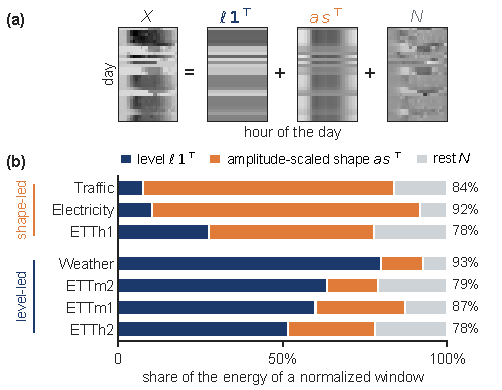
\includegraphics[width=\linewidth]{figures/token_energy.pdf}
\caption{窗口是一个水平项加一个按振幅缩放的形状。(a)~一个归一化的 Traffic 窗口（每天一行）及其在\equref{eq:three_parts}中的三个项。(b)~三个正交项的能量占比，在测试窗口上取平均；数字为前两项之和。橙色在三个数据集上占主导，深蓝在其余四个上占主导。}
\label{fig:token_energy}
\end{figure}

将周期序列的一个归一化窗口折叠成矩阵 $X\in\mathbb R^{D\times H}$，每个周期一行，周期内每个位置一列，该位置称为其\emph{相位}（第\ref{sec:method}节）。各行重复同一个模式，但并不精确：有些周期整体偏高，有些摆动更大。因此三个量就能描述一个窗口：\emph{形状} $s\in\mathbb R^H$，即所有周期共有的模式；每个周期的\emph{水平} $\ell_k$，即其均值；每个周期的\emph{振幅} $a_k$，即其围绕水平摆动的幅度。每个周期等于它的水平加上它的振幅乘以形状，于是
\begin{equation}
X=\ell\,\one^\top+a\,s^\top+N ,
\label{eq:three_parts}
\end{equation}
即一个\emph{水平项}加一个\emph{按振幅缩放的形状}，其中 $\ell,a\in\mathbb R^D$，$N$ 为余项。这里 $\ell$ 为各周期均值，$s$ 均值为零、均方根为一，$a\,s^\top$ 是对周期内部分 $X-\ell\,\one^\top$ 的最佳秩一拟合，因此三项两两正交。去掉余项后，窗口的秩至多为二：它的各列位于 $\ell$ 与 $a$ 张成的平面中，各行位于 $\one$ 与 $s$ 张成的平面中。

真实窗口与这一形式很接近：在每个数据集上，水平项与按振幅缩放的形状承载窗口 78\% 至 93\% 的能量（图\ref{fig:token_energy}）。由于窗口经过归一化，水平项衡量的是水平在窗口内漂移的程度，而不是整体偏移。哪一项占主导取决于数据：按振幅缩放的形状在 Electricity、Traffic 和 ETTh1 上占主导，水平项在其余四个数据集上占主导。因此两项都不能舍弃。

\fakeparagraph{要点}
\emph{窗口是一个水平项加一个按振幅缩放的形状，每个基准数据集都需要这两项。}预测模型的标记必须承载形状、水平与振幅。}

\begin{figure}[t]
\centering
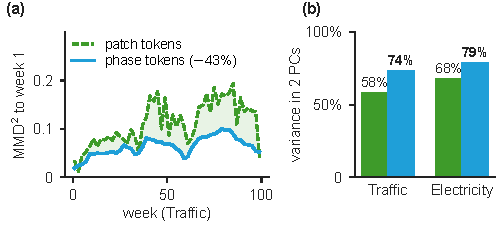
\includegraphics[width=\linewidth]{figures/token_geometry.pdf}
\caption{\blue{相位标记稳定且紧凑地承载形状。(a)~Traffic 上每周的标记相对第一周的漂移（MMD$^2$）；越低越稳定。(b)~前两个主成分所解释的方差；越高越紧凑。绿色：分块标记；蓝色：相位标记。}}
\label{fig:phase_token_comparison}
\end{figure}

\subsection{\blue{形状：相位标记稳定地承载它}}
\label{sec:mot_stability}

\blue{哪种标记能承载这些部分？由\equref{eq:three_parts}，\emph{分块标记}是 $X$ 的一行，$\ell_k\one+a_k\,s$：形状与 $\one$ 一起张成它所在的平面。\emph{相位标记}是一列，$\ell+s_p\,a$：它位于 $\ell$ 与 $a$ 张成的平面中，形状只通过权重 $s_p$ 决定它在平面中的位置。标记还必须\emph{稳定地}承载其部分：当该部分变化时，标记应停留在基于过去窗口拟合的模型所预期的位置。

考虑形状的变化，例如通勤习惯改变时，每个周期的早晚高峰都同样地移动。相位标记只在其平面内移动；分块标记所在的平面则会转动。真实数据同时呈现了这两种效应。}

\fakeparagraph{洞察 1：在 Traffic 上，相位标记的漂移更小}
\blue{在 Traffic 上，我们用平方最大均值差异（MMD$^2$）~\citep{ouyang2021mmd} 衡量每周的标记相对第一周的标记漂移了多远；相位标记的漂移比分块标记低 43\%（图\ref{fig:phase_token_comparison}(a)）。}

\fakeparagraph{洞察 2：相位标记更紧凑}
\blue{前两个主成分在 Traffic 上解释相位标记 74\% 的方差，在 Electricity 上解释 79\%，而分块标记分别只有 58\% 和 68\%（图\ref{fig:phase_token_comparison}(b)）：相位标记集中在 $\ell$ 与 $a$ 张成的平面中，而分块标记与输入窗口一样可以从周期中的任一相位开始，因此散布在形状的许多平移副本上。}

\blue{定理\ref{thm:stability}对任意低秩窗口 $X=AG^\top+N$ 证明了这一机制；\equref{eq:three_parts}是其中 $A=[\ell,\,a]$、$G=[\one,\,s]$ 的情形，公共形状变化把 $X$ 变为 $XS^\top$。证明见电子补充材料。}

\begin{theorem}[\blue{相位标记的稳定性}]
\label{thm:stability}
\blue{设 $X=AG^\top+N$，其中 $A$、$G$ 与 $SG$ 的秩均为 $r$；设 $X'=XS^\top+R$，$R$ 为小扰动。记 $\mathcal U_r$ 与 $\mathcal V_r$ 分别为相位标记与分块标记的前 $r$ 维子空间，$d$ 为子空间之间的距离，$\delta_{\min}>0$ 为信号的谱间隙，$\eta=C(\|N\|_2+\|NS^\top\|_2+\|R\|_2)/\delta_{\min}$，$C$ 为普适常数。则}
\begin{enumerate}[leftmargin=2em]
\item \blue{$d\big(\mathcal U_r(X),\mathcal U_r(X')\big)\le\eta$：相位标记保持其子空间，无噪声时严格不变；}
\item \blue{$d\big(\mathcal V_r(X),\mathcal V_r(X')\big)\ge d\big(\mathrm{Col}(G),\mathrm{Col}(SG)\big)-\eta$：形状变化使 $\one$ 与 $s$ 张成的平面转动多少，分块标记就移动多少。}
\end{enumerate}
\end{theorem}

\fakeparagraph{要点}
\blue{\emph{相位标记稳定地承载形状；分块标记做不到。}另一面是：相位标记的平面由 $\ell$ 与 $a$ 张成，因此仍会移动相位标记的，是水平或振幅的变化。}

\blue{
\subsection{水平与振幅：需要自己的标记}
\label{sec:mot_changes}

\begin{figure}[t]
\centering
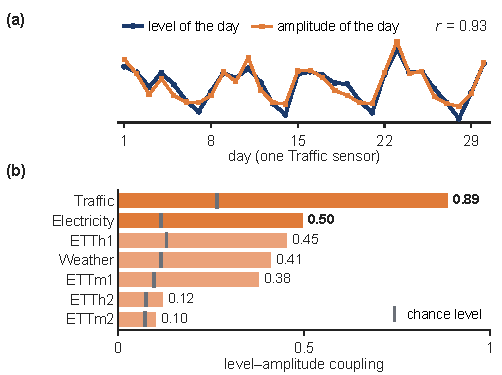
\includegraphics[width=\linewidth]{figures/coupling.pdf}
\caption{越繁忙的日子摆动越大。(a)~某个 Traffic 传感器每天的水平与振幅，已标准化。(b)~各数据集测试窗口上的水平–振幅耦合；深色：两个传感器网络；刻度：偶然水平。}
\label{fig:coupling}
\end{figure}

在一个窗口内，水平与振幅逐周期变化：一条道路有些天比另一些天更繁忙，而在繁忙的日子里，早晚高峰远高于夜间（图\ref{fig:coupling}(a)）。因此，随着窗口向前移动，它会带来新的轨迹 $\ell$ 与 $a$。在折叠后的窗口中，这两种变化为
\begin{equation}
\underbrace{X+\delta\,\one^\top}_{\text{水平漂移}},
\qquad
\underbrace{X+\operatorname{diag}(\alpha\ell)\,(X-\ell\,\one^\top)}_{\text{跟随水平的振幅}},
\label{eq:cycle_axis_changes}
\end{equation}
其中 $\delta\in\mathbb R^D$ 平移各周期的水平，$\alpha$ 决定摆动随水平增长的强度。它们把 $\ell$ 换成 $\ell+\delta$，把 $a$ 换成 $(\one+\alpha\ell)\odot a$。两者改变的恰是张成相位标记平面的那两条轨迹，因此一般都会移动这个平面。只读取相位标记的模型必须在每个窗口中重新估计水平与振幅，第\ref{sec:theory}节表明，在固定权重下，它只能在两个可由权重计算的包络之内做到这一点。因此，水平与振幅需要自己的标记。

不过，二者不必拥有两个彼此独立的标记。把这两种变化结合起来，加上噪声和以随机游走漂移的水平，就得到原始序列的一个简单季节模型，
\begin{equation}
X_{kp}=\ell_k+(1+\alpha\ell_k)\,s_p+e_{kp},
\qquad
\ell_k=\ell_{k-1}+\eta_k,
\label{eq:mult_model}
\end{equation}
其中形状 $s$ 均值为零、均方根为一，噪声为高斯噪声。当 $\alpha=0$ 时，它是加性季节随机游走模型；当 $\alpha\neq0$ 时，摆动随水平增大（$\alpha>0$）或减小（$\alpha<0$），我们仿照 Holt--Winters 预测的乘性形式~\citep{winters1960forecasting}，称之为乘性模型。此时振幅 $\one+\alpha\ell$ 是水平的函数，对水平的预测也就给出了振幅，因此一个水平标记就能同时驱动两者。洞察~3 表明真实数据正是如此。

\fakeparagraph{洞察 3：振幅跟随水平}
在图\ref{fig:coupling}(a) 的 Traffic 窗口中，30 天的水平与振幅同起同落（$r=0.93$）。为检验每个数据集，我们在每个通道的每个测试窗口中计算二者的相关系数，并在每个通道的各窗口上对带符号的相关系数取平均，使偶然相关相互抵消；再对这些通道平均值的绝对值取平均，因为符号在通道内稳定，但在 ETTh1 和 ETTm1 上因通道而异。所得的\emph{水平–振幅耦合}在七个基准数据集中的五个上远高于其偶然水平（即把水平与振幅取自不同窗口时的同一统计量），并在两个传感器网络上最强：Traffic 上为 0.89，Electricity 上为 0.50（图\ref{fig:coupling}(b)）。ETTh2 和 ETTm2 的耦合最弱，但在这两个数据集上水平本身主导窗口（图\ref{fig:token_energy}(b)），因此同样需要水平标记。电子补充材料给出细节，并表明训练期与验证期上的排序相同。

\fakeparagraph{要点：一个形式，三个标记}
\emph{水平与振幅逐周期变化，而且振幅跟随水平。}因此，\equref{eq:three_parts}的每个部分都有自己的标记（表\ref{tab:three_tokens}）：形状由相位标记承载，水平由每周期一个数的水平标记承载，振幅由从水平标记计算出的振幅标记承载。每个部分一个标记，就没有留给网络去解开的混杂；三个部分全部覆盖，就没有任何遗漏。第\ref{sec:method}节为每个标记构建一条小通路，第\ref{sec:theory}节说明为什么每条通路都是必要的，以及为什么三者合起来就足够。

\begin{table}[t]
\centering
\caption{一个形式，三个标记。}
\label{tab:three_tokens}
\footnotesize
\setlength{\tabcolsep}{2.5pt}
\begin{tabular}{@{}l l p{0.2\linewidth} p{0.31\linewidth} l@{}}
\toprule
部分 & 因子 & 如何变化 & 紧凑形式 & 标记 \\
\midrule
形状 & $s$ & 在每个周期中同样变化 & 一个向量；相位标记保持其子空间（定理~\ref{thm:stability}） & 相位 \\
水平 & $\ell$ & 逐周期变化 & 每周期一个数 & 水平 \\
振幅 & $a$ & 随水平变化 & 每周期一个数，由水平计算（洞察~3） & 振幅 \\
\bottomrule
\end{tabular}
\end{table}
}
